\documentclass[11pt, twoside, pdftex]{article}

% This include all the settings that we should use for the document
\newcommand{\PDFTitle}{DESim Installation Guide}
\newcommand{\commonPath}{../../../Tutorials/Common}
\input{\commonPath/Docs/defaulttext.tex}
\input{\commonPath/Docs/preamble.tex}

%%%%%%%%%%%%%%%%%%%%%%%%%
% Add title
\newcommand{\doctitle}{DESim Installation Guide}
\newcommand{\dochead}{DESim Installation Guide}
% Usually no need to change these two lines
\title{\fontfamily{phv}\selectfont{\doctitle} }
\chead{ \small{\textsc{\bfseries \dochead} } }
% Customizations
\newenvironment{ctabbing}%
{\begin{center}\begin{minipage}{\textwidth}\begin{tabbing}}
{\end{tabbing}\end{minipage}\end{center}}

%%%%%%%%%%%%%%%%%%%%%%%%%
% Allows multiple figures per page

\renewcommand\floatpagefraction{.9}
\renewcommand\topfraction{.9}
\renewcommand\bottomfraction{.9}
\renewcommand\textfraction{.1}   
\setcounter{totalnumber}{50}
\setcounter{topnumber}{50}
\setcounter{bottomnumber}{50}
\raggedbottom

\definecolor{AppleGreen}{rgb}{0.55, 0.71, 0.0}
\newcommand{\green}[1]{{\color{AppleGreen}\sf{#1}}}

\renewcommand{\versnum}{~} %version number quartus/AMP

%%%%%%%%%%%%%%%%%%
%%% DOCUMENT START
\begin{document}
\begin{table}
    \centering
    \begin{tabular}{p{5cm}p{4cm}}
        \hspace{-3cm}
        &
        \raisebox{1\height}{\parbox[h]{0.5\textwidth}{\Large\fontfamily{phv}\selectfont{\textsf{\doctitle}}}}
    \end{tabular}
    \label{tab:logo}
\end{table}

\colorbox[rgb]{0,0.384,0.816}{\parbox[h]{\textwidth}{\color{white}\textsf{\textit{\textBar}}}}

\thispagestyle{plain}
 
\section{Introduction}

The {\it DESim}\textsuperscript{\textregistered} application provides a 
graphical user interface (GUI) that represents some of the 
input devices and output displays on a DE-series board that features
an Altera\textsuperscript{\textregistered} FPGA 
device. This GUI serves as a "front end" to the {\it ModelSim} (or {\it Questa}) 
HDL simulator. Hence, before using {\it DESim} you must first install {\it ModelSim} 
(or {\it Questa}) onto your computer.  Instruction for installing {\it ModelSim} 
(or {\it Questa}) are provided on the \texttt{Software} tab of the website
{\small \href{https://www.fpgacademy.org/tools.html} {FPGAcademy.org}}.

After installing your Simulator software, you should follow the process described below
to download and configure the {\it DESim}\textsuperscript{\textregistered} application.
From the \texttt{DESim} section of {\small \href{https://www.fpgacademy.org/tools.html}
{FPGAcademy.org}}, download onto your computer the file named {\it DESim.zip}.
Then, {\it extract} the contents of this {\it archive} into a folder of your choice.
For example, if you use a folder named 
\texttt{C:$\backslash$DESim}, then it will appear as shown in Figure~\ref{fig:install}. 

\section{Configuring the DESim Application}
\label{sec:config}
To start the {\it DESim} application, you execute the {\it batch} script named 
{\it DESim\_run.bat}, which is listed in Figure~\ref{fig:install}. But you should
first open this script file to {\it configure} the {\it DESim} application. Since it is a 
plain ASCII text file, you can open {\it DESim\_run.bat} using any editor of your choice. 
A few of the key statements in this file are shown in Figure~\ref{fig:bat}.

\begin{figure}[h]
	\begin{center}
        \setlength{\fboxsep}{0pt}
        \fbox{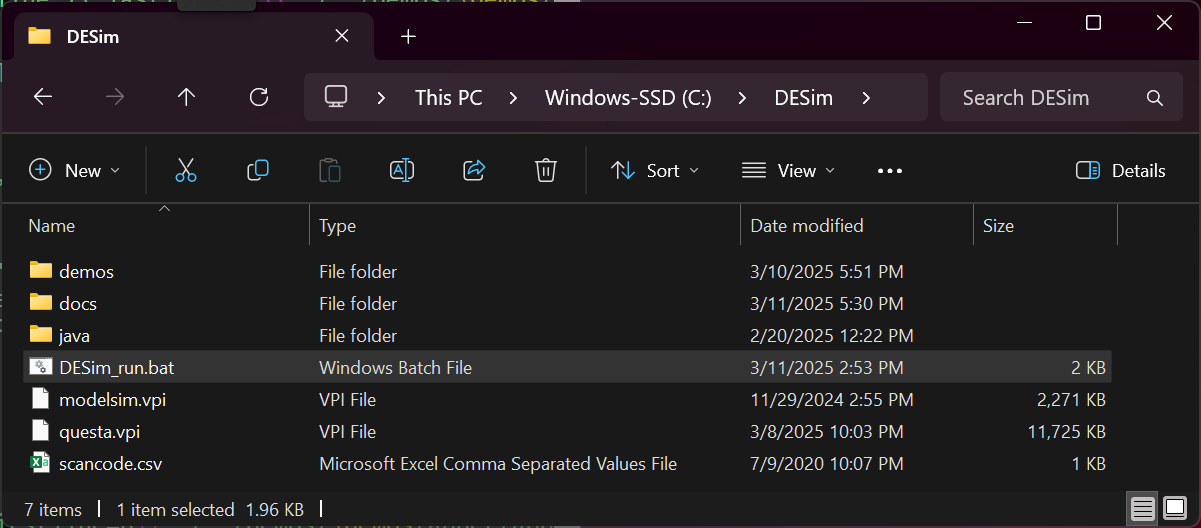
\includegraphics[width = \textwidth]{figures/Extract.png}}
	\end{center}
		  \caption{The {\it DESim} folder.}
	\label{fig:install}
\end{figure}

\begin{figure}[H]
\begin{center}
    \begin{minipage}[t]{16.75 cm}
\lstinputlisting[language=command.com, numbers=left, commentstyle=\color{brown}, keepspaces=tue, linerange={1-7,15-16, 25-27}, consecutivenumbers=false, escapechar=|]{figures/DESim_run.bat}
    \end{minipage}
		  \caption{The {\it DESim\_run.bat} script.}
	\label{fig:bat}
\end{center}
\end{figure}

Lines 5 and 6 of Figure~\ref{fig:bat} allow you to specify whether you are using the
{\it ModelSim} or {\it Questa} simulator. If you are using {\it ModelSim}, which is the
default, then this setting should be left unchanged. But if you are using {\it Questa},
then insert \texttt{REM} to ``comment-out'' Line 5 and remove the \texttt{REM} keyword 
on Line 6 to select {\it Questa}. 

The default setting provided in Line 15 starts the {\it DESim} GUI. This statement assumes
that your Simulator can be found without specifying its location in the filesystem,
meaning that the Simulator's location is included in your operating system's {\it Path}
environment variable.  If your computer is set up in this way, then you should keep this
setting.  But if your {\it Path} environment variable does not include the location of
your Simulator, then you should ``comment-out'' with \texttt{REM} Line 15 and instead use
the statement in Line 25 to start {\it DESim}.  Remove the \texttt{REM} from Line 25 and
replace \texttt{<SimulatorPath>} with the actual location of the folder where you have
installed your Simulator.

In most cases you will not need to make any other changes
\footnote{If your {\it Questa} (or {\it ModelSim}) version requires a license, then you should
make an \texttt{LM\_LICENSE\_FILE} environment variable that specifies the location of your
{\it license file}. But if you cannot set this variable, then the {\it DESim\_run.bat} file 
describes a command-line option that can be used to specify your license-file location.}
to the {\it DESim\_run.bat} file, and you 
should be ready to execute this batch script to start the {\it DESim} application. Complete
instructions for using {\it DESim} are provided in the {\it docs} folder listed in 
Figure~\ref{fig:install}, and also in the 
\texttt{DESim} section of {\small \href{https://www.fpgacademy.org/tools.html}
{FPGAcademy.org}}.

% Copyright and Trademark

\input{\commonPath/Docs/copyright.tex}

\end{document}
